\begin{center}
    \section{Lista de Exercícios}    
\end{center}

\subsection{Questões}

\begin{quest}
    A Física utiliza de modelos abstratos para explicar os fenômenos da natureza, o modelo Partícula (ou corpuscular) e o modelo Ondulatório são dois exemplos destes modelos. Cite as principais diferenças entre o modelo Partícula e o Modelo Ondulatório.
\end{quest}
\begin{quest}
    Por que o fenômeno da refração não pode ser explicado pelo Modelo Partícula?            
\end{quest}
% \begin{quest}
%     Por que o céu é azul durante o dia e alaranjado/avermelhado ao final da tarde? (Pesquise.)
% \end{quest}
\begin{quest}
    Se o índice de refração $n_1$ cujo o qual tem-se origem um feixe de luz é obrigatoriamente o ar, qual deve ser a direção de propagação do feixe refratado em um meio qualquer de índice de refração $n_2$?
\end{quest}
\begin{quest}
    A partir da \autoref{fig:questao-5} a seguir, responda as questões
    \vspace*{30pt}
    \begin{figure}[ht!]
        \centering
        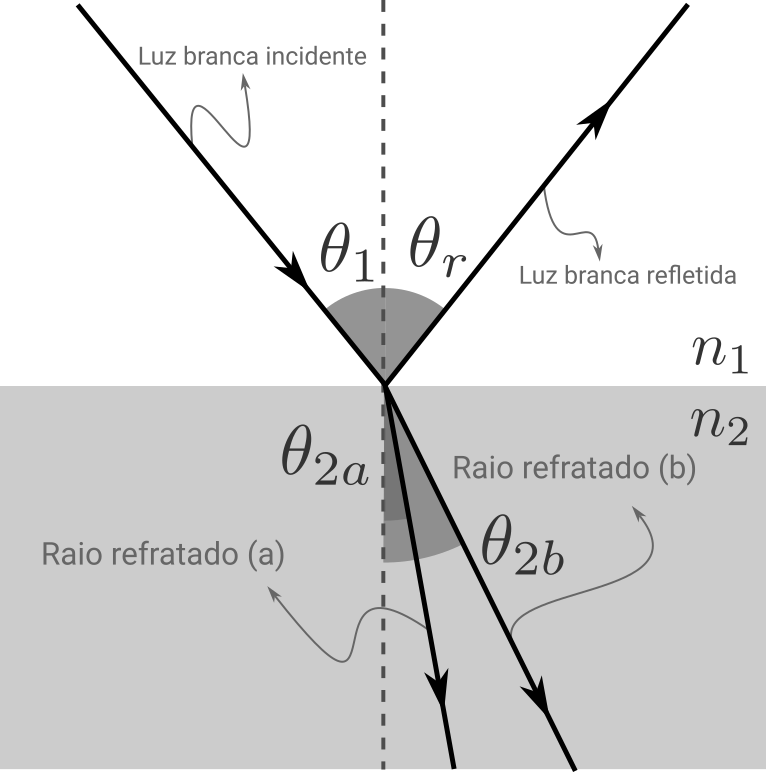
\includegraphics[width=.6\textwidth]{img/questao-5.png}
        \caption{Dispersão da luz branca em um meio material de índice de refração $n_2$}
        \label{fig:questao-5}  
    \end{figure}
    \vspace*{20pt}
    \begin{enumerate}[label=\alph *)]
        \item Se $\theta_r$ é o ângulo da luz refletida, o que pode-se afirmar sobre $\theta_r$ com relação ao ângulo de incidência $\theta_1$?
        \item Dentre os índices de refração $n_1$ e $n_2$ qual é o maior? (Justifique!)
        \item Supondo que ocorra o fenômeno de dispersão máxima entre os raios refratados, qual deve ser a cor do raio refratado ($a$) e do raio refratado ($b$), respectivamente? (Justifique!)
    \end{enumerate}        
\end{quest}

\subsection{Problemas}

\begin{prob}
    Um feixe de luz monocromático incide sobre uma superfície de separação entre dois meios. O meio 1 (incidente) possui índice de refração $n_1$, o meio 2 (refratado) possui índice de refração $n_2$. Se os ângulos de incidência e de refração são respectivamente $\theta_1=30^{\circ}$ e $\theta_2=45^{\circ}$, determine a razão entre $n_1$ e $n_2$.
\end{prob}
\begin{prob}
    Uma raio de luz monocromático propaga-se de um meio cujo o índice de refração vale $n_1$, para um outro meio de índice de refração $n_2=1,00$, formando com a normal à superfície ângulos de $\theta_1=30^{\circ}$ (incidente) e $\theta_2=45^{\circ}$ (refratado). Qual a velocidade da luz no meio incidente $n_1$?
\end{prob}
\begin{prob}(ENEM)
     A \autoref{fig:problema-3} representa um prisma óptico, constituído de um material transparente, cujo índice de refração é crescente com a frequência da luz que sobre ele incide. Um feixe luminoso, composto por luzes vermelha, azul e verde, incide na face $A$, emerge na face $B$ e, após ser refletido por um espelho, incide num filme para fotografia colorida, revelando três pontos.

    \vspace{20pt}
    \begin{figure}[ht!]
        \centering
        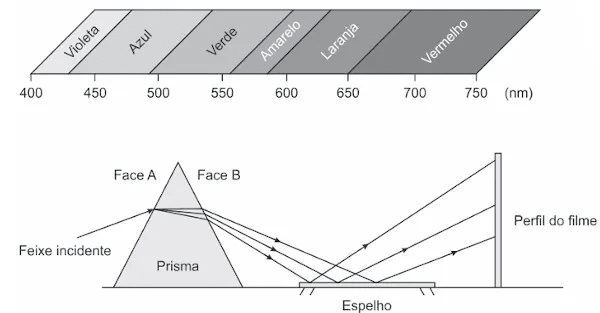
\includegraphics[width=.6\textwidth]{img/problema-3.png}
        \caption{Dispersão da luz em um prisma.}
        \label{fig:problema-3}                
    \end{figure}
    \vspace{20pt}
    \noindent Observando os pontos luminosos revelados no filme, de baixo para cima, constatam-se as seguintes cores:
    \begin{enumerate}[label=\alph *)]
        \item vermelha, verde, azul.
        \item verde, vermelha, azul.
        \item azul, verde, vermelha.
        \item verde, azul, vermelha.
        \item azul, vermelha, verde.
    \end{enumerate}
\end{prob}
\begin{prob}(ENEM)
    Alguns povos indígenas ainda preservam suas tradições realizando a pesca com lanças, demonstrando uma notável habilidade. Para fisgar um peixe em um lago com águas tranquilas o índio deve mirar abaixo da posição em que enxerga o peixe.

    \noindent Ele deve proceder dessa forma porque os raios de luz:
    \begin{enumerate}[label=\alph *)]
        \item refletidos pelo peixe não descrevem uma trajetória retilínea no interior da água.
        \item emitidos pelos olhos do índio desviam sua trajetória quando passam do ar para a água.
        \item espalhados pelo peixe são refletidos pela superfície da água.
        \item emitidos pelos olhos do índio são espalhados pela superfície da água.
        \item refletidos pelo peixe desviam sua trajetória quando passam da água para o ar.
    \end{enumerate}
\end{prob}
\begin{prob}(UDESC)
    Considere uma lâmina de vidro de faces paralelas imersa no ar. Um raio luminoso propaga-se no ar e incide em uma das faces da lâmina, segundo um ângulo  $\theta$ em relação à direção normal ao plano da lâmina. O raio é refratado nesta face e refletido na outra face, que é espelhada. O raio refletido é novamente refratado na face não espelhada, voltando a propagar-se no ar. Sendo $n_{a}$ e $n_{v}$   respectivamente, os índices de refração da luz no ar e no vidro, o ângulo de refração $\alpha$ que o raio refletido forma no vidro, com a direção normal ao plano da lâmina, ao refratar-se pela segunda vez, obedece à equação:
    \begin{enumerate}[label=\alph *)]
        \item $n_{v}\sin\alpha=n_{a}\sin(\theta /2)$
        \item $\alpha=\theta$
        \item $\sin\alpha=\cos\theta$
        \item $n_v\sin\alpha=n_a\sin\theta$
        \item $n_a\sin\alpha=n_v\sin\theta$
    \end{enumerate}
\end{prob}